% Minimal DFA of the words whose third letter from the end is a (generated by figs_c3ch01.py).
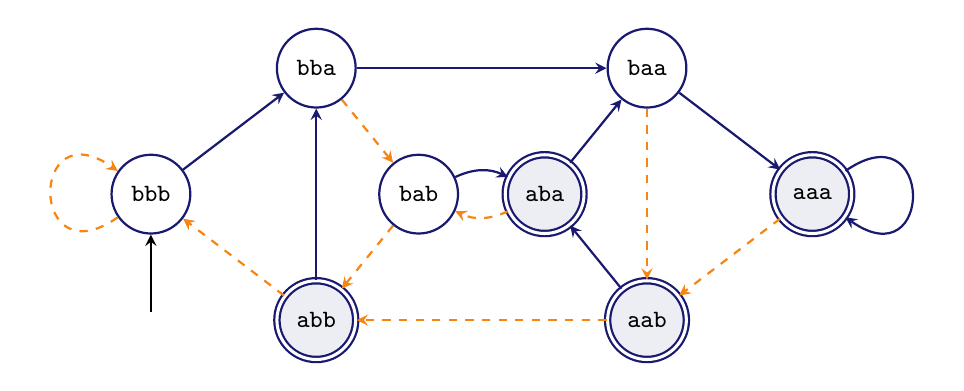
\begin{tikzpicture}[>=stealth,x=1cm,y=1cm,
  st/.style={circle,draw=MidnightBlue,thick,minimum size=10mm,inner sep=0pt,font=\small\ttfamily},
  acc/.style={st,double,double distance=1.1pt,fill=MidnightBlue!8}]
\node[st] (bbb) at (-4.2,0) {bbb};
\node[st] (bba) at (-2.1,1.6) {bba};
\node[acc] (abb) at (-2.1,-1.6) {abb};
\node[st] (bab) at (-0.8,0) {bab};
\node[acc] (aba) at (0.8,0) {aba};
\node[st] (baa) at (2.1,1.6) {baa};
\node[acc] (aab) at (2.1,-1.6) {aab};
\node[acc] (aaa) at (4.2,0) {aaa};
\draw[->,thick] (-4.2,-1.5) -- (bbb);
\draw[->,MidnightBlue,thick] (bbb) -- (bba);
\draw[->,BurntOrange,thick,dashed] (bbb) to[out=215,in=145,looseness=6] (bbb);
\draw[->,MidnightBlue,thick] (bba) -- (baa);
\draw[->,BurntOrange,thick,dashed] (bba) -- (bab);
\draw[->,MidnightBlue,thick] (abb) -- (bba);
\draw[->,BurntOrange,thick,dashed] (abb) -- (bbb);
\draw[->,MidnightBlue,thick] (bab) to[bend left=25] (aba);
\draw[->,BurntOrange,thick,dashed] (bab) -- (abb);
\draw[->,MidnightBlue,thick] (aba) -- (baa);
\draw[->,BurntOrange,thick,dashed] (aba) to[bend left=25] (bab);
\draw[->,MidnightBlue,thick] (baa) -- (aaa);
\draw[->,BurntOrange,thick,dashed] (baa) -- (aab);
\draw[->,MidnightBlue,thick] (aab) -- (aba);
\draw[->,BurntOrange,thick,dashed] (aab) -- (abb);
\draw[->,MidnightBlue,thick] (aaa) to[out=35,in=-35,looseness=6] (aaa);
\draw[->,BurntOrange,thick,dashed] (aaa) -- (aab);
\end{tikzpicture}
